\documentclass[11pt,a4paper]{article}
\usepackage[utf8]{inputenc}
\usepackage[portuguese]{babel}
\usepackage[T1]{fontenc}
\usepackage[ddmmyyyy]{datetime}
\usepackage[margin=2cm]{geometry}
\usepackage{amsfonts}
\usepackage{amsmath}
\usepackage{amssymb}
\usepackage{amsthm}
\usepackage[citestyle=authortitle]{biblatex}
\usepackage{csquotes}
\usepackage{graphicx}
\usepackage{mathtools}
\usepackage{thmtools}
\usepackage{titling}
\usepackage{xcolor}
\usepackage{enumitem}
\usepackage[unicode]{hyperref}

\pdfsuppressptexinfo=7

\graphicspath{{e-folio/e-folio-a/imagem}}
\addbibresource{bibliografia.bib}

% Ambientes de provas e demonstrações
\newtheorem{proposition}{Proposição}[section]
\renewcommand\qedsymbol{\textbf{q.e.d.}}

% Dados
\author{Carlos Augusto Gonçalves Collaço e Pinto Machado}
\newcommand{\numeroEstudante}{2200909}
\newcommand{\UC}{Elementos de Análise Infinitesimal I}
\newcommand{\codigoUC}{21030}
\newcommand{\docentes}{Maria João Oliveira}
\newcommand{\curso}{Licenciatura em Matemática e Aplicações}
\newcommand{\turma}{2}
\newcommand{\anoLectivo}{2023-2024}
\date{\today}

\pagenumbering{arabic}

\hypersetup{
	pdfsubject={\UC},
	pdftitle={E-fólio A - \numeroEstudante},
	pdfauthor={Carlos Pinto Machado},
	pdfproducer={},
	pdfcreator={}
}

\makeindex

\newcommand{\exercicio}{
	\addtocounter{section}{1}
	\setcounter{subsection}{0}
	\section*{\arabic{section}}
	\addcontentsline{toc}{section}{Exercício \arabic{section}}
}


\begin{document}

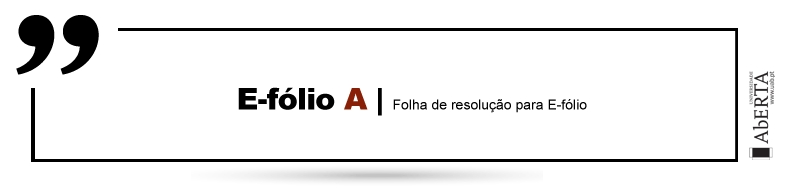
\includegraphics[width=\textwidth]{e-folio-a.jpg}

\paragraph{\textbf{UNIDADE CURRICULAR:}} \UC

\paragraph{\textbf{CÓDIGO:}} \codigoUC

\paragraph{\textbf{DOCENTE:}} \docentes

\paragraph{\textbf{NOME:}} \theauthor

\paragraph{\textbf{N.º DE ESTUDANTE:}} \numeroEstudante

\paragraph{\textbf{CURSO:}} \curso

\paragraph{\textbf{DATA DE ENTREGA:}} \thedate


\clearpage

\exercicio{}

\begin{equation}
	\begin{cases}
		v_1 = 1 \\
		v_{n + 1} = \frac{v^2_n}{1 + v_n}, \quad n \in \mathbb{N}
	\end{cases}
\end{equation}

\begin{enumerate}[label=\arabic{section}.\arabic*.]
	\item
	      \begin{proposition}\label{prop:efa-1a}
		      Para qualquer $n \in \mathbb{N}$, tem-se que $0 < v_n\leq 1$.
	      \end{proposition}
	      \begin{proof}
		      \hfill\\
		      \begin{enumerate}[label=\arabic*.]
			      \item Começamos pelo caso $n = 1$, no qual tem-se que $v_1 = 1 \in]0, 1]$
			            , que é uma afirmação verdadeira.
			      \item Fixamos agora um $n \in \mathbb{N}$ e assumimos que
			            \begin{align*}
				                 & 0 < v_n \leq 1 \quad\quad \text{(Hipótese de Indução)}
				            \intertext{Queremos mostrar que:}
				                 & 0 < v_{n + 1} \leq 1 \quad \text{(Tese de Indução)}
				            \intertext{Procedemos ao Passo de indução, no qual
							com base na hipótese, tem-se que}
				                 & 0 < v_n \leq 1 \implies 0 < v_n^2 \leq 1               \\
				                 & 0 < v_n \leq 1 \iff \; 1 < 1 + v_n
				            \intertext{Que nos permite, deduzir que:}
				                 & 0 < v_n^2 \leq 1 < 1 + v_n                             \\
				            \iff & 0 < \frac{v_n^2}{1 + v_n} \leq \frac{1}{1 + v_n} < 1
				            \intertext{Dado que
					            $v_{n + 1} = \frac{v_n^2}{1 + v_n}$, podemos
					            concluir que está demonstrado que}
				                 & 0 < v_{n+1} \leq 1.
								 \intertext{Que nos permite concluir a nossa
									 demonstração da proposição, por indução,
									 no qual fica demonstrado que para $n \in
									 \mathbb{N}$, tem-se que $0 < v_n \leq
								 1$.}
			            \end{align*}
		      \end{enumerate}
	      \end{proof}
	\item
	      \begin{proposition}
		      A sucessão $(v_n)$ é monótona.
	      \end{proposition}
	      \begin{proof}
		      \; \\
		      De modo a verificar se a sucessão é monótona, vamos verificar se
		      $v_{n+1} - v_n$ é positivo ou negativo.
		      \begin{align*}
			      v_{n + 1} - v_n = \frac{v_n^2}{1 + v_n} - v_n
			      = \frac{v_n^2-v_n(1 + v_n)}{1 + v_n}
			      = -\frac{v_n}{1 + v_n}
		      \end{align*}
		      Com base na proposição \ref{prop:efa-1a}, do exercício anterior, tem-se que
		      \begin{align*}
			      0 < v_n \leq 1 \iff 1 < 1 + v_n \implies
			      v_{n + 1} - v_n = -\frac{v_n}{1 + v_n} < 0
		      \end{align*}
		      Que nos permite concluir que a sucessão $(v_n)$ é estritamente
		      decrescente, consequentemente monótona.\\
	      \end{proof}
	      \clearpage
	\item \hfill
	      \begin{enumerate}[label=\arabic{section}.\arabic{enumi}.\arabic*.]
			  \item \; \\
				  Pretende-se estudar a natureza da série, definida por:
		            \begin{equation}\label{eq:efa-1-3-1}
			            \sum_{n=1}^{\infty} v_n
		            \end{equation}
				  \begin{align*}
					  \intertext{Pela Proposição \ref{prop:efa-1a}, do
					  exercício 1.1, tem-se que}
					  0 < v_n \leq 1 \iff &1 < 1 + v_n \\
					  \iff &
					  0 < \frac{v_n}{1+v_n} < 1.
					  \intertext{Donde se tem que:}
					  \lim_{n \to \infty} \left|\frac{v_{n + 1}}{v_n}\right|
					  &=
					  \lim_{n \to \infty}
					  \left|\frac{\frac{v_n^2}{1+v_n}}{v_n}\right|\\
					  &=
					  \lim_{n \to \infty}
					  \left|\frac{v_n^2}{v_n(1+v_n)}\right|\\
					  &=
					  \lim_{n \to \infty}
					  \left|\frac{v_n}{1+v_n}\right| < 1\\
					  \intertext{Deste modo concluímos, pelo Critério
						  D'Alembert(Teorema 7, alínea 1), que a série é
					  absolutamente convergente.}
				  \end{align*}
			\item \; \\
				  Pretende-se estuda a natureza da série, definida por:
				  \begin{equation}\label{eq:efa-1-3-2}
			            \sum_{n=1}^{\infty} \frac{v_n}{1 + v_n}
		          \end{equation}
				  Vamos começar por verificar se os termos gerais
				  da série $\sum_{n=1}^{\infty} \frac{v_n}{1 + v_n}$  e da
				  série $\sum_{n=1}^{\infty} v_n$, do exercício anterior, são
				  assimptoticamente iguais
				  \footcite[pág. 384, Definição 7]{Santos2016}:
				  \begin{align*}
					  \lim_{n \to \infty} \frac{\frac{v_n}{1+vn}}{v_n} =
					  \lim_{n \to \infty} \frac{1}{1 + v_n} = 1 \implies
					  \frac{v_n}{1 + v_n} \sim v_n
				  \end{align*}
				  Pelo Critério da
				  comparação(Teorema 6, alínea 1)\footcite[pág.
				  595]{Santos2016}, dado que
				  $\sum_{n=1}^{\infty} \frac{v_n}{1 + v_n}$ e
				  $\sum_{n=1}^{\infty} v_n$ são ambas séries de termos
				  não negativos, e assimptoticamente iguais podemos concluir 
				  que as séries têm a mesma natureza. Logo a série
				  $\sum_{n=1}^{\infty} \frac{v_n}{1 + v_n}$ é absolutamente
				  convergente.
	      \end{enumerate}
\end{enumerate}

\clearpage
\exercicio{}

\begin{equation}\label{eq:efa-2}
	\sum_{n=0}^{\infty} \frac{1}{1 + \alpha^{2n}}
\end{equation}

\paragraph{} Seja $\alpha \in \mathbb{R}$, pretende-se determinar os valores
de $\alpha$ para qual a série, definida em \ref{eq:efa-2}, converge.

\begin{align*}
	\intertext{Começamos por observar que}
	\alpha^{2n}
	&= (\alpha^n)^2 \geq 0
	\intertext{Se $|\alpha| < 1$, tem-se que}
	\lim_{n \to \infty} 1 + \alpha^{2n}
	&= 1
	\iff \lim_{n \to \infty} \frac{1}{1 + a^{2n}} = 1.
	\intertext{Se $|\alpha| = 1$, tem-se que}
	\lim_{n \to \infty} 1 + \alpha^{2n}
	&= 2
	\iff \lim_{n \to \infty} \frac{1}{1 + a^{2n}} = \frac{1}{2}.
	\intertext{Se $|\alpha| > 1$, tem-se que}
	\lim_{n \to \infty} 1 + \alpha^{2n}
	&= +\infty
	\iff \lim_{n \to \infty} \frac{1}{1 + a^{2n}} = 0.
\end{align*}

\paragraph{}Pela alínea 1 do Teorema
4\footcite[pág. 579]{Santos2016}, a série só converge se o termo
geral convergir para 0. Logo, a série
$\sum_{n=0}^{\infty} \frac{1}{1+\alpha^{2n}}$ é convergente para
$\alpha \in ]-\infty, -1[ \cup ]1, +\infty[$.






\clearpage

\nocite{*}
\printbibliography[heading=bibintoc,title={Bibliografia}]

\end{document}
